\documentclass[10pt]{article}
\usepackage[margin=0.58in]{geometry}
\usepackage{booktabs,enumitem,fancyhdr,graphicx,tabularx,titlesec}
\usepackage[hidelinks]{hyperref}
\graphicspath{{docs/lessons/assets/}{../assets/}}
\hypersetup{pdftitle={ADK Lesson 057: Inert Escape-room Console},
 pdfauthor={Kevin Shanahan},
 pdfsubject={Atomic copied-clue composition, stop precedence, attributed audit, and inert presentation intent},
 pdflang={en-US}}
\pagestyle{fancy}\fancyhf{}
\lhead{\textsc{ADK Lesson 057}}\rhead{Inert Escape-room Console}
\cfoot{\thepage}\setlength{\headheight}{14pt}
\setlength{\parindent}{0pt}\setlength{\parskip}{2.5pt}
\setlist{nosep,leftmargin=1.45em}
\titleformat{\section}{\Large\bfseries}{\thesection}{0.5em}{}
\newcommand{\lessonbox}[1]{\begin{center}\fbox{\parbox{0.92\linewidth}{#1}}\end{center}}
\newcommand{\blankline}{\rule{0.72in}{0.4pt}}

\begin{document}
\small
\begin{center}
 {\Huge\bfseries Inert Escape-room Console}\\[3pt]
 {\Large Solve six clue stations without opening anything}\\[7pt]
 \fbox{\textbf{E0 POLICY COMPOSITION --- NO DOOR, LOCK, LATCH, LAMP, OR POWER PATH}}
\end{center}
\begin{tabularx}{\linewidth}{@{}>{\bfseries}l X >{\bfseries}l X@{}}
Lesson & 057 --- project & Time & 180--240 minutes\\
Prerequisites & Lessons 055 and 056 & Board & compile-only Mega replay\\
Evidence & named memory result cells & Boundary & copied values and inert intent\\
\end{tabularx}

\lessonbox{\textbf{Project boundary.} \texttt{InertEscapeConsole} owns a
fixed clue model and a fault-aware operator panel. It publishes only copied
lamp, presentation, and demonstration-latch intent. It owns no endpoint, pin,
interrupt, timer, display, storage medium, servo, relay, lamp, latch, door,
lock, or power path. It is not access control, confinement, egress, an
emergency release, a protective interlock, or a life-safety system.}

\section{Tour the six fictional stations}
Twelve copied clues form six fixed pairs. The family mapping is part of the
configuration digest; runtime input cannot rename or rearrange it.

\begin{center}
% ADK visual: pencil
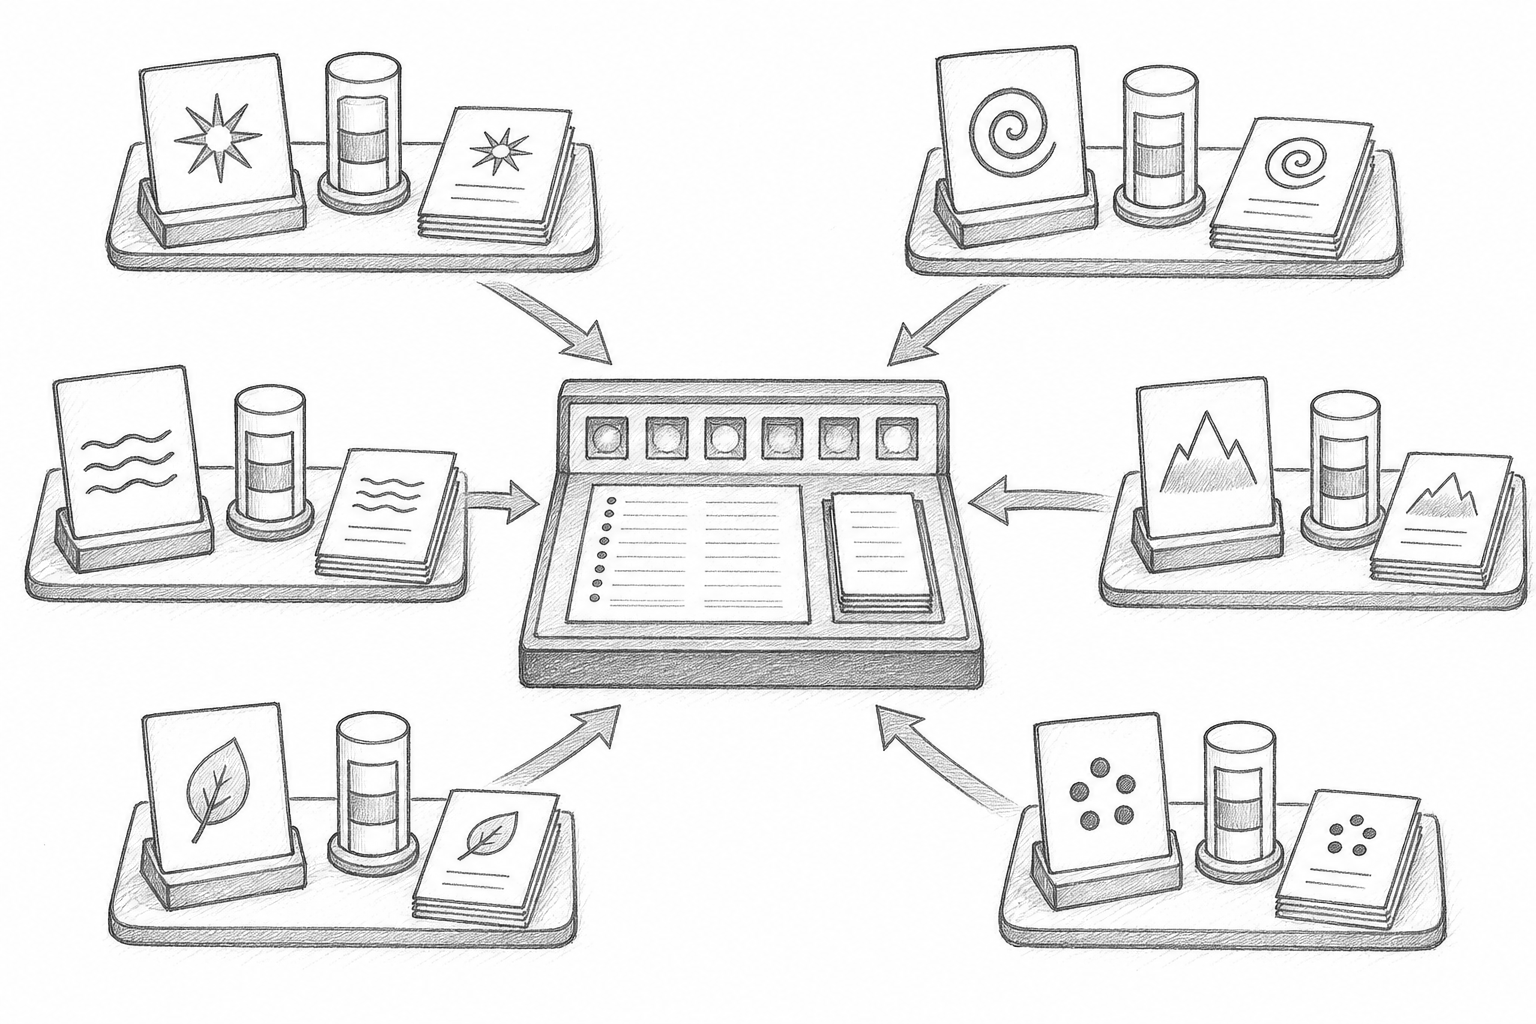
\includegraphics[width=0.98\linewidth,height=0.31\textheight,
 keepaspectratio]{057-six-station-console-pencil.png}

\small\textit{Alternative text: a graphite tabletop console is surrounded by
six clearly separate fictional stations, each with two symbolic clue cards.
Arrows carry their copied results to a central policy notebook. The adjacent
table gives the exact Sequence, Pattern, Orientation, Presence, Rhythm, and
Alignment mapping; no wiring, door, lock, or powered actuator is present.}
\end{center}

\begin{tabularx}{\linewidth}{@{}l l X@{}}
\toprule
Family & Clues & What the E0 replay observes\\
\midrule
Sequence & 0--1 & two copied categorical values and their provenance\\
Pattern & 2--3 & two independent evidence cells, never an inferred sensor\\
Orientation & 4--5 & symbolic categories, not a physical pose measurement\\
Presence & 6--7 & synthetic presence categories, not occupancy or identity\\
Rhythm & 8--9 & copied categories, not audio sampling or timing hardware\\
Alignment & 10--11 & synthetic alignment, not position or motion authority\\
\bottomrule
\end{tabularx}

Every family summary reports its clue IDs, completeness, and weakest quality.
It cannot grant solve authority. Only the complete twelve-rule DAG, qualified
stop evidence, panel state, audit state, and a deliberate
\texttt{prepareSolve()} can do that.

\section{Submit one complete atomic envelope}
\texttt{EscapeConsoleUpdate} carries one supplied time and presence-qualified
copies of the audit image, clue update, stop, control, audit acknowledgement,
diagnostic acknowledgement, presentation evidence, and solve preview.
Noncanonical absent values, malformed evidence, or a structurally invalid
image reject the whole envelope without mutation.

After structural validation, precedence is fixed:

\begin{enumerate}
 \item retained lifecycle, configuration, source, and timing faults;
 \item qualified stop assertion or an unreconciled stop transition;
 \item clue faults, stale evidence, contradiction, and invalid chords;
 \item corrupt or indeterminate audit state and presentation failure;
 \item ordinary panel audit or diagnostic acknowledgement;
 \item exact solve commit; and
 \item progress, confirmation, solved, or inactive presentation intent.
\end{enumerate}

There is no public clue, stop, acknowledge, solve, show, latch, or lamp call
whose caller-selected order can change that precedence.

\begin{center}
% ADK visual: pencil
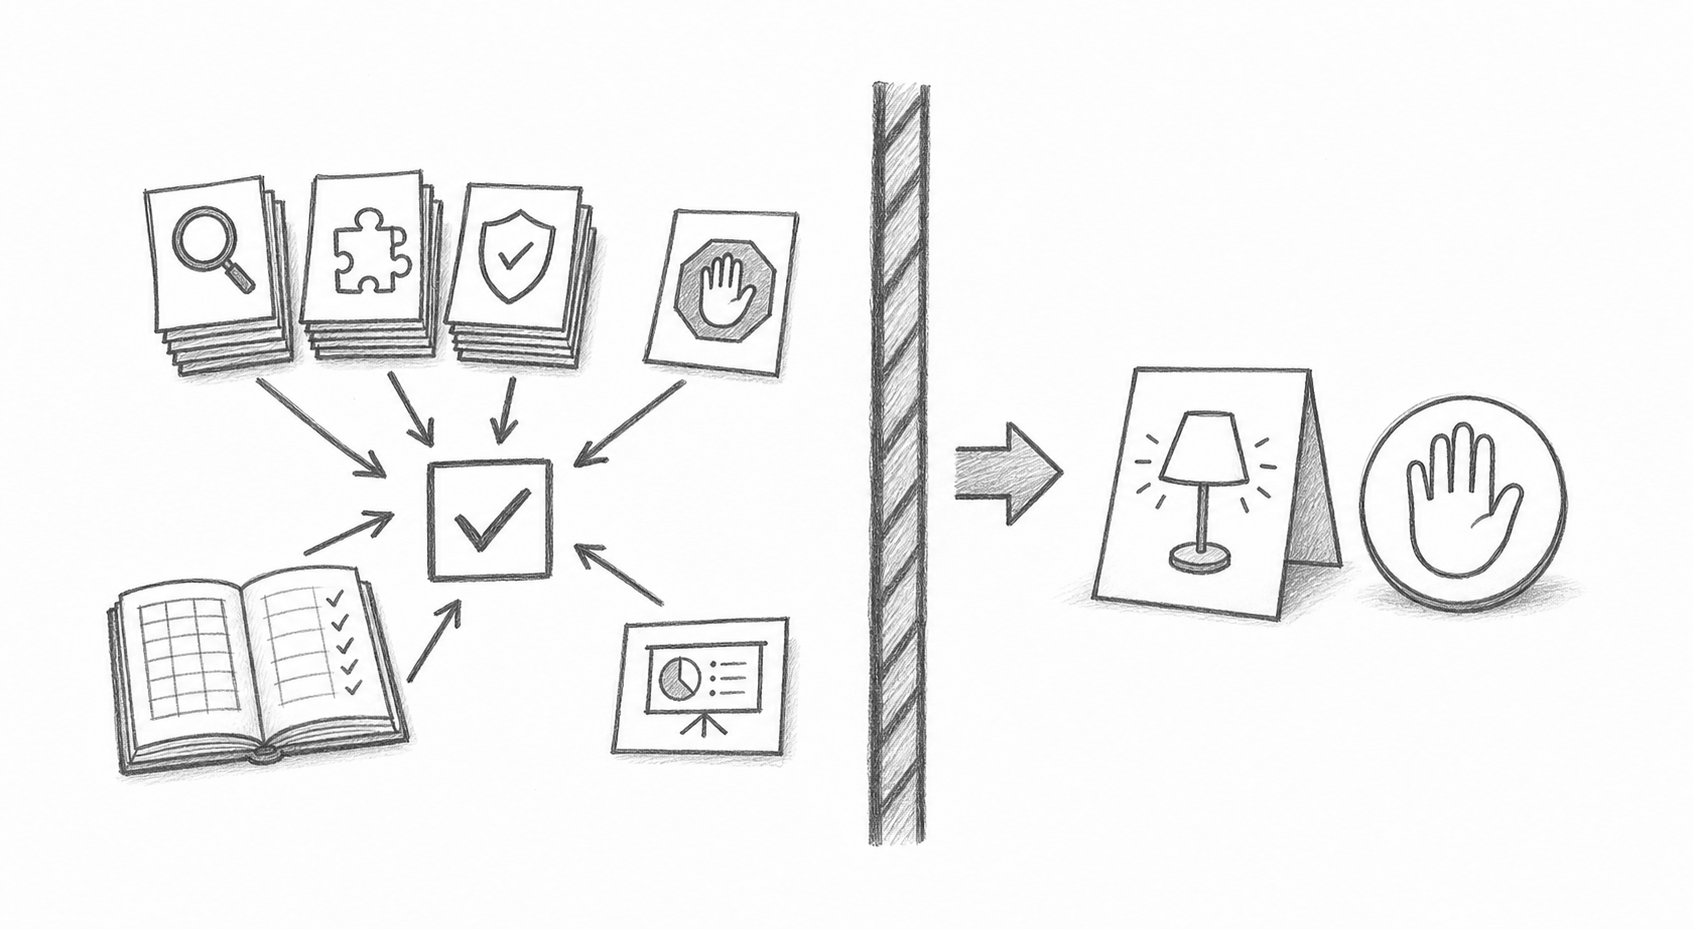
\includegraphics[width=0.98\linewidth,height=0.29\textheight,
 keepaspectratio]{057-atomic-solve-pencil.png}

\small\textit{Alternative text: a hand-drawn envelope contains clue, stop,
control, presentation, audit-image, acknowledgement, and solve-preview cards.
A graphite checklist validates the complete envelope before two child
notebooks and one parent result cell change together. A bold stop card diverts
the envelope to inactive latch and stopped lamp intent before the solve path.}
\end{center}

\section{Read predictions from named memory cells}
\begin{tabularx}{\linewidth}{@{}l X X@{}}
\toprule
Cell & Prediction & Interpretation\\
\midrule
six family cells & incomplete, then complete with weakest quality &
copied clue grouping only\\
constraint cell & exact clue generation and satisfied-rule mask &
fixed DAG result, not physical truth\\
panel cell & diagnostic, selected station, stop and audit disposition &
copied operator policy only\\
audit image & latest two canonical records & modeled memory, not persistence\\
lamp cell & off, ready, progress, confirmation, solved, fault, or stopped &
semantic presentation intent only\\
latch cell & inactive except one solved transaction &
request for an absent demonstration actuator\\
\bottomrule
\end{tabularx}

These volatile cells are the E0 non-Serial observation path. Compilation does
not prove that a powered Mega executed the sketch or that any physical
indicator displayed the result.

\section{Prepare and bind one solution}
\texttt{prepareSolve(operationId, now)} is the deliberate operator
confirmation. A selected panel cell, a Select control, or twelve satisfied
rules cannot silently substitute for this named call.

Preparation requires a solved retained clue generation, all six families
complete, fresh qualified deasserted stop evidence, no pending stop audit,
clear dominant diagnostics, and a canonical audit image that is
\texttt{Ready} or the exact empty-image \texttt{PrepareRequired} bootstrap.
It privately prepares the child \texttt{PuzzleSolved} record.

The returned preview binds:

\begin{itemize}
 \item parent owner token, lifecycle, configuration revision, and epoch;
 \item console generation, operation ID, policy digest, clue generation, and
       satisfied-rule mask; and
 \item the complete child audit preview, including its owner, lifecycle,
       sequence, slot, record, image digest, and predecessor.
\end{itemize}

\texttt{canCommit()} answers only whether those retained preview fields are
still live. It does not validate a later image or promise that a later
\texttt{update()} will commit. A foreign, stale, changed, consumed,
reset-invalidated, child-mismatched, or image-mismatched preview rejects.

\section{Commit parent and child together}
The caller models a write by copying the prepared child record into the
specified audit-image slot. A later complete envelope supplies that image,
the exact child acknowledgement nested in the parent preview, and the exact
parent preview.

The coordinator first prepares the complete proposed clue and panel states.
It recomputes families, diagnostics, presentation, latch intent, lamp intent,
policy identity, and every preview binding from those proposed values. Only
after every parent and child preflight succeeds do the infallible apply seams
mutate both children and publish one parent transition.

\begin{tabularx}{\linewidth}{@{}l X@{}}
\toprule
Collision in the same envelope & Required result\\
\midrule
stop assertion plus solve & stop wins; neither capability is consumed\\
clue becomes stale or contradictory plus solve & solve is suppressed\\
presentation fails plus solve & fault intent; no solved audit commit\\
invalid control chord plus solve & invalid chord; inactive latch intent\\
wrong or torn audit image plus solve & reject or fail closed; no partial state\\
exact canonical image and both previews & one \texttt{Solved} transition\\
\bottomrule
\end{tabularx}

Sequential best-effort mutation and rollback after an observable child change
are outside the design. If implementation ever needs either, stop promotion
and repair the architecture.

\section{Make stop and restart boring}
A default \texttt{stopped == false} value is not qualified evidence. Missing,
stale, faulted, or asserted stop evidence rejects solution preparation.
A qualified asserted observation publishes stopped intent and requires its
exact \texttt{StopAsserted} audit record. A later qualified deasserted
observation still leaves latch intent inactive until the exact newer
\texttt{StopReleased} record commits.

\begin{tabularx}{\linewidth}{@{}l X X@{}}
\toprule
Stage & Predict & Observe\\
\midrule
stop collides with solve & stopped dominates & inactive latch; no solved record\\
asserted record commits & stopped remains retained & canonical audit sequence\\
deassertion arrives & release still pending & inactive latch; pending audit\\
released record commits & ordinary puzzle policy resumes & canonical newer record\\
shutdown and initialize & blank volatile state & inactive/off; no image assumed\\
clean image replay & deterministic reconciliation & Ready or retained Stopped\\
torn image replay & fail closed & Corrupt or Indeterminate; inactive latch\\
\bottomrule
\end{tabularx}

Software stop is neither emergency stop nor power removal. Even a later
physical demonstration needs an independent means to remove load power.

\section{Run the deterministic console workbook}
\begin{enumerate}
 \item Initialize without an image. Predict inactive latch intent, lamp off,
       six incomplete families, and an unreconciled audit disposition.
 \item Supply every one of the \(2^{12}\) clue-presence masks. Confirm that
       each family becomes complete only when both mapped clues are eligible.
 \item Replay the twelve-rule chain from incomplete through solved. Inject
       stale, contradictory, source-faulted, wrong-source, future, regressed,
       and half-range-ambiguous evidence.
 \item Exercise all 16 low-nibble control masks. Confirm zero means no control,
       one bit means one control, and every multi-bit chord is invalid.
 \item Fail presentation, recover it with exact current-generation evidence,
       prepare its acknowledgement, and commit the attributed audit record.
 \item Prepare a solve from the empty-image bootstrap and from a normal Ready
       image. Mutate each parent and child preview field separately.
 \item Collide solve with stop, clue changes, presentation failure, invalid
       chord, audit ambiguity, and mismatched images. Prove no partial commit.
 \item Complete stop assertion and release audits, then restart from clean,
       torn, corrupt, indeterminate, and adjacent committed images.
 \item Replay two configured instances field-for-field and compare every
       snapshot and canonical audit field.
\end{enumerate}

\begin{tabularx}{\linewidth}{@{}X X X X X X@{}}
\toprule
stage & families & rule mask & panel & audit & latch/lamp\\
\midrule
\rule{0pt}{16pt}\blankline & \blankline & \blankline & \blankline & \blankline & \blankline\\[8pt]
\blankline & \blankline & \blankline & \blankline & \blankline & \blankline\\[8pt]
\blankline & \blankline & \blankline & \blankline & \blankline & \blankline\\
\bottomrule
\end{tabularx}

\section{Separate acquisition from safe state}
\textbf{Acquisition prediction and observation.} Canonical fixed
configuration, nonzero parent and child revisions and epochs, twelve source
identities, six exact family pairs, and a matching derived policy digest allow
initialization. Host tests inspect lifecycle generations, object bindings,
clue and panel snapshots, canonical audit fields, and distinct result cells.

\textbf{Acquisition interpretation.} This proves fixed-storage E0 policy
construction only. It does not acquire a sensor, control, stop circuit,
display, storage medium, lamp, latch, actuator, or power path.

\textbf{Safe-state prediction and observation.} Construction, failed
initialization, reset, shutdown, stop, fault, invalid evidence, audit
ambiguity, and restart begin or remain at inactive latch intent. Host tests
observe that copied state directly.

\textbf{Safe-state interpretation.} Inactive memory intent is not electrical
isolation, an emergency stop, a released exit, or proof of a physical latch,
lamp, or door state.

\section{Read the measured resource evidence}
The exact no-LTO maximum-composition Mega 2560 probe measures 34,978 bytes of
flash and 3,655 bytes of static SRAM.
\texttt{sizeof(InertEscapeConsole)} is exactly 1,024 bytes. Conservative
compiler evidence measures a 951-byte deepest synchronous stack path.
After adding a separate 128-byte interrupt reserve, the residual SRAM is
\(8192-3655-951-128=3458\) bytes.

The object, stack, static-SRAM, and residual values pass their targets. Flash
misses the 32,768-byte target but passes the reviewed 40,960-byte hard limit;
the fixed-capacity value-owned children and atomic parent/child path are
retained rather than weakening ownership or solve semantics. The checked-in
\texttt{escape-console-resource-check} binds the accepted target miss to this
exact measured tuple and review record.

These are compiler, linker, and conservative accounting results for exact
fixtures and a recorded toolchain. They are not runtime high-water
measurements, physical timing evidence, or proof of any hardware endpoint.
Rerun the probe after any source, toolchain, optimization, library, fixture,
buffer, or aggregate-composition change.

\section{Keep powered work outside E0}
E1 must separately qualify the exact passive clue and control inputs,
low-voltage current-limited presentation hardware, complete pin and electrical
data, pull policy, source identity, named observation points, unpowered wiring
inspection, failure injection, and bench acceptance. Servo, relay, latch,
lock, door, and other powered actuation remain physically absent.

E2 may consider only a restrained no-load demonstration servo or an inert
current-limited low-voltage relay-and-lamp fixture, with independent physical
load-power removal and recorded bench acceptance. It must never attach to a
door, gate, lock, occupied enclosure, alarm, emergency lighting, egress route,
or life-safety system. No person, animal, property, or safe exit may depend on
this project.

\section{Record the E0 result}
\begin{itemize}
 \item policy digest: \blankline\quad final clue generation: \blankline
 \item satisfied-rule mask: \blankline\quad final audit sequence: \blankline
 \item solved transaction: \blankline\quad stop-dominance result: \blankline
 \item restart result: \blankline\quad inactive safe-state result: \blankline
\end{itemize}

\end{document}
